\documentclass[article,12pt]{elsarticle}
\usepackage[spanish]{babel}
\usepackage[utf8]{inputenc}
\usepackage{amssymb}
\usepackage{flushend}
\usepackage{float}
\usepackage{anysize}
\usepackage{amsmath}
\usepackage{amsfonts}
\usepackage{dcolumn}
\usepackage{amsthm}
\usepackage{caption}
\usepackage{float}
\usepackage{subfigure}
\usepackage{graphicx}
\usepackage{lmodern}
\usepackage{booktabs}
\usepackage{color}
\usepackage{longtable}
\usepackage{rotating}
\usepackage{etoolbox}
\usepackage{comment}
\usepackage{pdflscape}
\usepackage{booktabs}


\begin{document}

\begin{frontmatter}
    \title{Laboratorio de Fenómenos Colectivos \\  Tarea de tensión Superficial} \\
    \author{Andrés López González$^1$} %Aquí va el nombre de los integrantes que participaron en el informe.
    \address{$^1$ Facultad de Ciencias, Universidad Nacional Autónoma de México, M\'exico CDMX.}
\end{frontmatter}

\section{Montaje experimental}

Se utilizó un soporte universal con un tubo suspendido de forma ortogonal a él ayudándonos de una nuez. Este tubo sostenía una pinza de tres dedos con un dinamómetro colgando. En el extremo del dinamómetro se fijó un anillo metálico con un hilo en forma de "X" que nos ayudaba a mantener el equilibrio, debajo de este montaje, una plataforma metálica ajustable sostenía un recipiente con agua. El recipiente se elevaba lentamente hasta que el anillo metálico entraba en contacto con la superficie del agua.

El objetivo del experimento era medir la fuerza necesaria para separar el anillo de la superficie del agua, obteniendo así la tensión superficial a partir de la variación de la fuerza registrada por el dinamómetro.


\section{Datos utilizados y cálculo de la tensión superficial:}
Los valores experimentales de la fuerza \( F_d \) y el peso del anillo \( Mg \) se registraron (Tabla 3 en el documento). Estos datos permiten aplicar el método de mínimos cuadrados forzando a la pendiente \( m_0 = 1 \), lo cual implica calcular la ordenada al origen \( b \) con la ecuación:

\[
b = \frac{1}{N} \sum_{i} (y_i - m_0 x_i)
\]

Aquí, \( y_i = F_d \) y \( x_i = Mg \). \( b \) representa la componente de la fuerza atribuida a la tensión superficial, mientras que \( m_0 x_i \) es la contribución debida al peso del anillo.

La incertidumbre de \( b \) se calcula como el valor máximo entre dos métodos:  
\begin{enumerate}
\item Máxima distancia vertical entre los puntos y la recta ajustada (\( \delta b \) por la ecuación (11)).
\item Propagación de incertidumbre considerando \( \delta b = \delta y + m_0 \delta x \) (ecuación (13)).
\end{enumerate}

\section{Resultados obtenidos:}
Con los datos proporcionados, el valor calculado para la ordenada al origen por el profesor fue:

\[
b = (0.0133 \pm 0.005) \, \text{N}
\]

Mientras en mi caso posterior a aplicar la regresión lineal a nuestra tabla $mg-F_d$ obtuvimos lo siguiente:\\

\begin{table}[h]
\centering
\begin{tabular}{|l|l|}
\hline
\textit{\textbf{mg (N)}} & \textit{\textbf{$F_d$ (N)}} \\ \hline
0.076                    & 0.092                       \\ \hline
0.085                    & 0.102                       \\ \hline
0.095                    & 0.112                       \\ \hline
0.105                    & 0.122                       \\ \hline
0.125                    & 0.142                       \\ \hline
0.135                    & 0.155                       \\ \hline
\end{tabular}
\caption{Tabla registrada}
\end{table}\\

Siendo el gráfico el siguiente con $b=0.01252762 \pm 0.005$ \\

\begin{figure}[h]
    \centering
    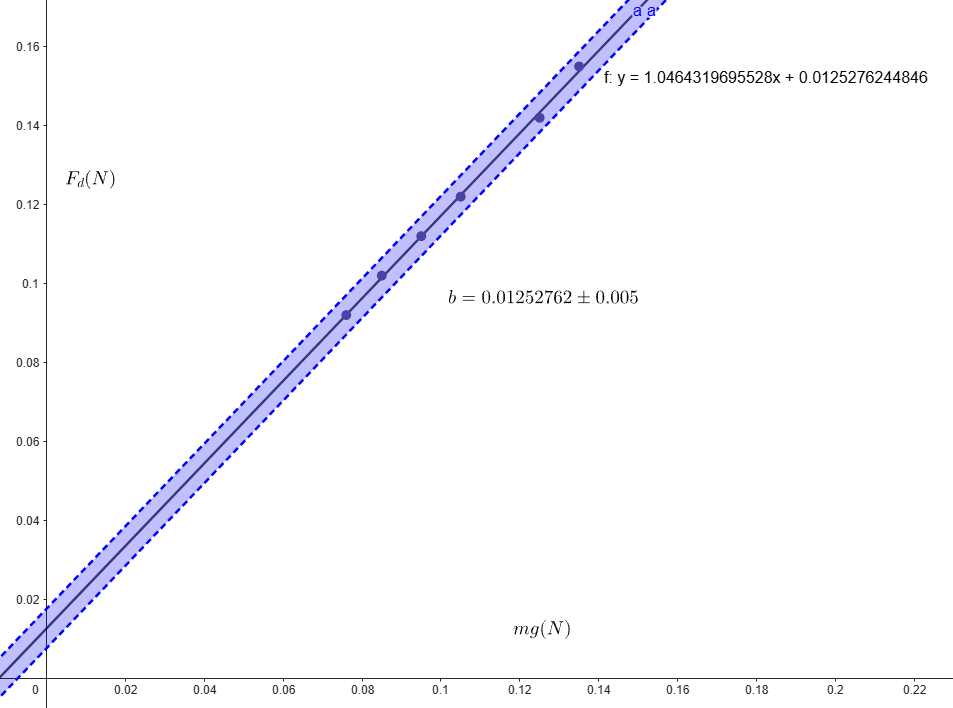
\includegraphics[width=1\linewidth]{Regression.png}
    \caption{Regresión lineal para mis valores}
    \label{fig:enter-label}
\end{figure}\\

La tensión superficial \( \tau \) del agua se deduce de la relación:

\[
\tau = \frac{b}{\pi (\phi_e + \phi_i)}
\]

Donde \( \phi_e \) y \( \phi_i \) son los diámetros externo e interno del anillo. Con propagación de incertidumbre:

\[
\delta \tau / \tau = \delta b / b + \frac{2 \delta v}{\phi_e + \phi_i}
\]

Se reportó finalmente:

\[
\tau = 0.0536898 \, \text{N/m} \pm 44\%
\]


\end{document}

